\documentclass[10pt, conference, compsocconf]{IEEEtran}
% Add the compsocconf option for Computer Society conferences.

% *** MISC UTILITY PACKAGES ***
%
%\usepackage{ifpdf}
% Heiko Oberdiek's ifpdf.sty is very useful if you need conditional
% compilation based on whether the output is pdf or dvi.
% usage:
% \ifpdf
%   % pdf code
% \else
%   % dvi code
% \fi
% The latest version of ifpdf.sty can be obtained from:
% http://www.ctan.org/tex-archive/macros/latex/contrib/oberdiek/
% Also, note that IEEEtran.cls V1.7 and later provides a builtin
% \ifCLASSINFOpdf conditional that works the same way.
% When switching from latex to pdflatex and vice-versa, the compiler may
% have to be run twice to clear warning/error messages.

% *** CITATION PACKAGES ***
%
\usepackage{cite}
% cite.sty was written by Donald Arseneau
% V1.6 and later of IEEEtran pre-defines the format of the cite.sty package
% \cite{} output to follow that of IEEE. Loading the cite package will
% result in citation numbers being automatically sorted and properly
% "compressed/ranged". e.g., [1], [9], [2], [7], [5], [6] without using
% cite.sty will become [1], [2], [5]--[7], [9] using cite.sty. cite.sty's
% \cite will automatically add leading space, if needed. Use cite.sty's
% noadjust option (cite.sty V3.8 and later) if you want to turn this off.
% cite.sty is already installed on most LaTeX systems. Be sure and use
% version 4.0 (2003-05-27) and later if using hyperref.sty. cite.sty does
% not currently provide for hyperlinked citations.
% The latest version can be obtained at:
% http://www.ctan.org/tex-archive/macros/latex/contrib/cite/
% The documentation is contained in the cite.sty file itself.

% *** GRAPHICS RELATED PACKAGES ***
%
\ifCLASSINFOpdf
  \usepackage[pdftex]{graphicx}
  % declare the path(s) where your graphic files are
  % \graphicspath{{../pdf/}{../jpeg/}}
  % and their extensions so you won't have to specify these with
  % every instance of \includegraphics
  % \DeclareGraphicsExtensions{.pdf,.jpeg,.png}
\else
  % or other class option (dvipsone, dvipdf, if not using dvips). graphicx
  % will default to the driver specified in the system graphics.cfg if no
  % driver is specified.
  % \usepackage[dvips]{graphicx}
  % declare the path(s) where your graphic files are
  % \graphicspath{{../eps/}}
  % and their extensions so you won't have to specify these with
  % every instance of \includegraphics
  % \DeclareGraphicsExtensions{.eps}
\fi

% *** MATH PACKAGES ***
%
\usepackage[cmex10]{amsmath}
\usepackage{amsfonts}   % Added by P.Avesani
% A popular package from the American Mathematical Society that provides
% many useful and powerful commands for dealing with mathematics. If using
% it, be sure to load this package with the cmex10 option to ensure that
% only type 1 fonts will utilized at all point sizes. Without this option,
% it is possible that some math symbols, particularly those within
% footnotes, will be rendered in bitmap form which will result in a
% document that can not be IEEE Xplore compliant!

% *** SPECIALIZED LIST PACKAGES ***
%
\usepackage[noend]{algorithmic}
% algorithmic.sty was written by Peter Williams and Rogerio Brito.
% This package provides an algorithmic environment fo describing algorithms.
% You can use the algorithmic environment in-text or within a figure
% environment to provide for a floating algorithm. Do NOT use the algorithm
% floating environment provided by algorithm.sty (by the same authors) or
% algorithm2e.sty (by Christophe Fiorio) as IEEE does not use dedicated
% algorithm float types and packages that provide these will not provide
% correct IEEE style captions. The latest version and documentation of
% algorithmic.sty can be obtained at:
% http://www.ctan.org/tex-archive/macros/latex/contrib/algorithms/
% There is also a support site at:
% http://algorithms.berlios.de/index.html
% Also of interest may be the (relatively newer and more customizable)
% algorithmicx.sty package by Szasz Janos:
% http://www.ctan.org/tex-archive/macros/latex/contrib/algorithmicx/




% *** ALIGNMENT PACKAGES ***
%
\usepackage{array}
% Frank Mittelbach's and David Carlisle's array.sty patches and improves
% the standard LaTeX2e array and tabular environments to provide better
% appearance and additional user controls. As the default LaTeX2e table
% generation code is lacking to the point of almost being broken with
% respect to the quality of the end results, all users are strongly
% advised to use an enhanced (at the very least that provided by array.sty)
% set of table tools. array.sty is already installed on most systems. The
% latest version and documentation can be obtained at:
% http://www.ctan.org/tex-archive/macros/latex/required/tools/


%\usepackage{mdwmath}
%\usepackage{mdwtab}
% Also highly recommended is Mark Wooding's extremely powerful MDW tools,
% especially mdwmath.sty and mdwtab.sty which are used to format equations
% and tables, respectively. The MDWtools set is already installed on most
% LaTeX systems. The lastest version and documentation is available at:
% http://www.ctan.org/tex-archive/macros/latex/contrib/mdwtools/


% IEEEtran contains the IEEEeqnarray family of commands that can be used to
% generate multiline equations as well as matrices, tables, etc., of high
% quality.


%\usepackage{eqparbox}
% Also of notable interest is Scott Pakin's eqparbox package for creating
% (automatically sized) equal width boxes - aka "natural width parboxes".
% Available at:
% http://www.ctan.org/tex-archive/macros/latex/contrib/eqparbox/





% *** SUBFIGURE PACKAGES ***
%\usepackage[tight,footnotesize]{subfigure}
% subfigure.sty was written by Steven Douglas Cochran. This package makes it
% easy to put subfigures in your figures. e.g., "Figure 1a and 1b". For IEEE
% work, it is a good idea to load it with the tight package option to reduce
% the amount of white space around the subfigures. subfigure.sty is already
% installed on most LaTeX systems. The latest version and documentation can
% be obtained at:
% http://www.ctan.org/tex-archive/obsolete/macros/latex/contrib/subfigure/
% subfigure.sty has been superceeded by subfig.sty.



%\usepackage[caption=false]{caption}
%\usepackage[font=footnotesize]{subfig}
% subfig.sty, also written by Steven Douglas Cochran, is the modern
% replacement for subfigure.sty. However, subfig.sty requires and
% automatically loads Axel Sommerfeldt's caption.sty which will override
% IEEEtran.cls handling of captions and this will result in nonIEEE style
% figure/table captions. To prevent this problem, be sure and preload
% caption.sty with its "caption=false" package option. This is will preserve
% IEEEtran.cls handing of captions. Version 1.3 (2005/06/28) and later 
% (recommended due to many improvements over 1.2) of subfig.sty supports
% the caption=false option directly:
%\usepackage[caption=false,font=footnotesize]{subfig}
%
% The latest version and documentation can be obtained at:
% http://www.ctan.org/tex-archive/macros/latex/contrib/subfig/
% The latest version and documentation of caption.sty can be obtained at:
% http://www.ctan.org/tex-archive/macros/latex/contrib/caption/




% *** FLOAT PACKAGES ***
%
%\usepackage{fixltx2e}
% fixltx2e, the successor to the earlier fix2col.sty, was written by
% Frank Mittelbach and David Carlisle. This package corrects a few problems
% in the LaTeX2e kernel, the most notable of which is that in current
% LaTeX2e releases, the ordering of single and double column floats is not
% guaranteed to be preserved. Thus, an unpatched LaTeX2e can allow a
% single column figure to be placed prior to an earlier double column
% figure. The latest version and documentation can be found at:
% http://www.ctan.org/tex-archive/macros/latex/base/



%\usepackage{stfloats}
% stfloats.sty was written by Sigitas Tolusis. This package gives LaTeX2e
% the ability to do double column floats at the bottom of the page as well
% as the top. (e.g., "\begin{figure*}[!b]" is not normally possible in
% LaTeX2e). It also provides a command:
%\fnbelowfloat
% to enable the placement of footnotes below bottom floats (the standard
% LaTeX2e kernel puts them above bottom floats). This is an invasive package
% which rewrites many portions of the LaTeX2e float routines. It may not work
% with other packages that modify the LaTeX2e float routines. The latest
% version and documentation can be obtained at:
% http://www.ctan.org/tex-archive/macros/latex/contrib/sttools/
% Documentation is contained in the stfloats.sty comments as well as in the
% presfull.pdf file. Do not use the stfloats baselinefloat ability as IEEE
% does not allow \baselineskip to stretch. Authors submitting work to the
% IEEE should note that IEEE rarely uses double column equations and
% that authors should try to avoid such use. Do not be tempted to use the
% cuted.sty or midfloat.sty packages (also by Sigitas Tolusis) as IEEE does
% not format its papers in such ways.





% *** PDF, URL AND HYPERLINK PACKAGES ***
%
\usepackage{url}
% url.sty was written by Donald Arseneau. It provides better support for
% handling and breaking URLs. url.sty is already installed on most LaTeX
% systems. The latest version can be obtained at:
% http://www.ctan.org/tex-archive/macros/latex/contrib/misc/
% Read the url.sty source comments for usage information. Basically,
% \url{my_url_here}.



%===========moi them vao =====================
\usepackage{graphicx}
\graphicspath{{figures/}}
%===========moi them vao =====================

% *** Do not adjust lengths that control margins, column widths, etc. ***
% *** Do not use packages that alter fonts (such as pslatex).         ***
% There should be no need to do such things with IEEEtran.cls V1.6 and later.
% (Unless specifically asked to do so by the journal or conference you plan
% to submit to, of course. )

\newcommand{\Ivec}[1]{\mbox{\boldmath $#1$}}
\newcommand{\argmin}{\operatornamewithlimits{argmin}}
\newcommand{\argmax}{\operatornamewithlimits{argmax}}
\newcommand{\sgn}{\operatorname{{\mathrm sgn}}}
\newcommand{\mean}{\operatornamewithlimits{mean}}
\newcommand{\Bin}{\operatorname{{\mathrm Bin}}}
\newcommand{\Beta}{\operatorname{{\mathrm Beta}}}
\newcommand{\Gammadist}{\operatorname{{\mathrm Gamma}}}
\newcommand{\Uniform}{\operatorname{{\mathrm Uniform}}}

% correct bad hyphenation here
\hyphenation{op-tical net-works semi-conduc-tor}

%% % Squeeze space to fit 4 pages constraint:
%% % \linespread{0.97}
%% % or
%% \setlength{\parskip}{0pt}
%% \setlength{\parsep}{0pt}
%% \setlength{\headsep}{0pt}
%% \setlength{\topskip}{0pt}
%% \setlength{\topmargin}{0pt}
%% \setlength{\topsep}{0pt}
%% \setlength{\partopsep}{0pt}
%% % \linespread{0.982}
\linespread{0.98}

\usepackage{hyperref}

\begin{document}
%
% paper title
% can use linebreaks \\ within to get better formatting as desired
% \title{The Dissimilarity Approximation for Tractography}
\title{Mapping Tractographies}

% author names and affiliations
% use a multiple column layout for up to two different
% affiliations

% \author{\IEEEauthorblockN{Authors Name/s per 1st Affiliation (Author)}
% \IEEEauthorblockA{line 1 (of Affiliation): dept. name of organization\\
% line 2: name of organization, acronyms acceptable\\
% line 3: City, Country\\
% line 4: Email: name@xyz.com}
% \and
% \IEEEauthorblockN{Authors Name/s per 2nd Affiliation (Author)}
% \IEEEauthorblockA{line 1 (of Affiliation): dept. name of organization\\
% line 2: name of organization, acronyms acceptable\\
% line 3: City, Country\\
% line 4: Email: name@xyz.com}
% }

\author{\IEEEauthorblockN{Thien Bao Nguyen\IEEEauthorrefmark{1}\IEEEauthorrefmark{2},
     Emanuele Olivetti\IEEEauthorrefmark{1}\IEEEauthorrefmark{2}, and Paolo Avesani\IEEEauthorrefmark{1}\IEEEauthorrefmark{2},
% %    , \emph{Member}, \emph{IEEE}
\\
     email: \url{tbnguyen@fbk.eu}, \url{olivetti@fbk.eu}, \url{avesani@fbk.eu}\\
 }
 \IEEEauthorblockA{\IEEEauthorrefmark{1}NeuroInformatics Laboratory (NILab),
 Fondazione Bruno Kessler, Trento, Italy}
 \IEEEauthorblockA{\IEEEauthorrefmark{2}Centro Interdipartimentale Mente e Cervello (CIMeC),
 Universit\`a di Trento, Italy}
% \IEEEauthorblockA{\IEEEauthorrefmark{3}SPL Lab,
% Brigham and Women's Hospital, Harvard Medical School, MA, USA}
}



% conference papers do not typically use \thanks and this command
% is locked out in conference mode. If really needed, such as for
% the acknowledgment of grants, issue a \IEEEoverridecommandlockouts
% after \documentclass

% for over three affiliations, or if they all won't fit within the width
% of the page, use this alternative format:
% 
%\author{\IEEEauthorblockN{Michael Shell\IEEEauthorrefmark{1},
%Homer Simpson\IEEEauthorrefmark{2},
%James Kirk\IEEEauthorrefmark{3}, 
%Montgomery Scott\IEEEauthorrefmark{3} and
%Eldon Tyrell\IEEEauthorrefmark{4}}
%\IEEEauthorblockA{\IEEEauthorrefmark{1}School of Electrical and Computer Engineering\\
%Georgia Institute of Technology,
%Atlanta, Georgia 30332--0250\\ Email: see http://www.michaelshell.org/contact.html}
%\IEEEauthorblockA{\IEEEauthorrefmark{2}Twentieth Century Fox, Springfield, USA\\
%Email: homer@thesimpsons.com}
%\IEEEauthorblockA{\IEEEauthorrefmark{3}Starfleet Academy, San Francisco, California 96678-2391\\
%Telephone: (800) 555--1212, Fax: (888) 555--1212}
%\IEEEauthorblockA{\IEEEauthorrefmark{4}Tyrell Inc., 123 Replicant Street, Los Angeles, California 90210--4321}}




% use for special paper notices
%\IEEEspecialpapernotice{(Invited Paper)}




% make the title area
\maketitle


\begin{abstract}
  We developed a novel interactive system for human brain tractography
  segmentation to assist neuroanatomists in identifying white matter
  anatomical structures of interest from diffusion magnetic resonance
  imaging data (dMRI). The difficulty in segmenting and navigating
  tractographies lies in the very large number of \emph{streamlines},
  in the order of hundreds of thousands, that modern MR techniques
  provide. The novelty of our system resides in presenting a clustered
  version of the tractography to the user which interactively selects
  the clusters of interest to narrow down the initial tractography to
  a subset containing the anatomical structure. The set of streamlines
  of the selected clusters are then re-clustered in smaller clusters
  so that the user can refine the previous selection and then
  re-cluster again at a finer scale. This process is iterated until
  the union of the remaining clusters faithfully represent the desired
  structure. The proposed system adopts a solution to solve the
  computational issue of clustering a large number of streamlines
  under the strict time constraints requested by the interactive
  use. The solution consists in projecting the streamlines into a
  Euclidean space and then in adopting a state-of-the art scalable
  implementation of the $k$-means algorithm. We tested the proposed
  system on tractographies from amyotrophic lateral sclerosis (ALS)
  patients and healthy subjects to study the systematic differences
  within the corticospinal tract.
\end{abstract}

%%% Local Variables: 
%%% mode: latex
%%% TeX-master: "olivetti_boi"
%%% End: 


\begin{IEEEkeywords}
  tractography mapping, tractography registration; tract segmentation; dissimilarity
  representation; dMRI
\end{IEEEkeywords}


% For peer review papers, you can put extra information on the cover
% page as needed:
% \ifCLASSOPTIONpeerreview
% \begin{center} \bfseries EDICS Category: 3-BBND \end{center}
% \fi
%
% For peerreview papers, this IEEEtran command inserts a page break and
% creates the second title. It will be ignored for other modes.
\IEEEpeerreviewmaketitle


\section{Introduction}
\label{sec:introduction}
%the need of visualization data
To support human in analyzing and exploring large data, it is an important task to graphically present the data~\cite{yang2003interactive}. Users, in one side, have a requirements of looking at complex and intricate data to find out some facts or trends that are not esy to find. On the other side, they want to explore data in details to examine each data points. In fact, the overall premise is that users have a deeper understanding about their data when they interact with the presented information and view it at different levels of abstraction~\cite{roberts2007state}. During the last two decades, many interactive visualization techniques and system have been emerged~\cite{yang2003interactive,stroe2000scalable,fua2000structure}.
As large data sets become more and more common, with the oder over $1K$, it has been clear that most of the current visualization approaches lose their effectiness due to they have no ability to visualize and manage the large number of data points simultaneously. In this scenerio, clustering is considered a suitable method for understanding and to exploring large data~\cite{berkhin2006survey,bisson2012improving}. 
However, clustering usually results in one partition of the data, and this leads to the drawback because the validation process is not straightforward due to the lack of grouth truth data~\cite{candillier2006casade}. One solution for this is hierarchical clustering~\cite{johnson1967hierarchical}, which organizes data in an intutive and interpretable way, namely dendrogram, not only one partion as the traditional clustering methods.
%In such tructure, all the degree of generality are present 
This character allows users to explore in a simple way the clusters and the relationships between instances, leading to many applications for visulization~\cite{heard2009novel,landesberger2011visual,mahe2009graph}.
%what is the limitation of current visualization method to large data
Nevertheless, when dealing practically with a large size dendrogram, it becomes difficult since the number of leaves grows exponentially with the depth of the tree and makes users lose the overview of the whole dataset. To deal with this prolbem, many sugguestion have been approached~\cite{bisson2012improving,landesberger2011visual,furnas2006fisheye}. However, these methods are either display at one time only a subpart of the structure~\cite{landesberger2011visual,furnas2006fisheye}, or display whole dendrogram but rely on other clustering technique~\cite{bisson2012improving}.

%Contents of the paper
In this work, we propose a framework of offering a complete and interactive visualization of the large data. Our method allow users to apply his or her perceptual abilities to make sense of data. 
%We describe the algorithmic solutions we adopted in order to build the interactive visualization large data.  
The core of the problem is to obtain the multiple scales for representation large data in order to comply with the requirements of human interactive visualization. The proposed solution combines three steps. First, the dendrogram would be created by running the hierarchical clustering. Second, the \emph{goodness} function is used as a measurement to select the most relevant scales for representing the dendrogram. Lastly, we also evaluate the multipe scales based on a application deriven criteria, called \emph{split factor}. 

% tractography segmentation tool. The core of the problem is to obtain fast clustering of a large number of streamlines in order to comply with the requirements of human interaction. The proposed solution combines two state-of-the-art elements: first a recently proposed Euclidean embedding algorithm for streamlines, i.e. the dissimilarity representation with the scalable \emph{subset farthest first} (SFF) prototype selection policy~\cite{olivetti2012approximation}. This embedding provides fast and accurate vectorial representation of streamlines, needed by most of the clustering algorithms. Second, a recently proposed improvement of the $k$-means clustering algorithm called \emph{mini-batch} $k$-means~\cite{sculley2010web} (MBKM). This algorithm drastically reduces the convergence time to the actual clusters in case of large and very-large sets of objects. We also tested a further potential improvement, i.e. a recently proposed initialisation algorithm for the $k$-means family, called $k-means++$~\cite{arthur2007kmeans}. But we excluded it from the final system due to poor performance as illustrated in Section~\ref{sec:experiments}.

% Structure of the paper
The paper is organized as follows. Section~\ref{sec:methods} introduces the
algorithmic elements of the proposed method including hierarchical clustering, multiple scales choosing and quantitatively evaluating the goodness of the representation. In section~\ref{sec:experiments}, we describe details of the actual use of the proposed solution in the context of the tractgoraphy segmentation, provide figures to evaluate the viability of the proposed solution. We conclude with a summary of our contribution and open areas for future work in the last section~\ref{sec:conclusion}.
%  and are formally described
%We quantitatively describe the segmentation process and provide figures to evaluate the viability of the proposed solution. In Section~\ref{sec:discussion} we discuss the results and we show that the proposed solution is effective. We conclude by mentioning the future steps for the development of our software, called \emph{spaghetti}, and the open computational challenges that needs to be solved.



\section{Methods}
\label{sec:methods}
In the following we describe the elements that we evaluated in order
to build the proposed method. After introducing the notation we
formally describe the dissimilarity representation, i.e. a Euclidean
embedding for streamlines, and then we present the mini-batch
$k$-means algorithm. We conclude by reporting how we efficiently
compute the medoids of the clusters from the centroids.

\subsection{Notation}
\label{sec:notation}
Let $X \in \mathcal{X}$ be a streamline, i.e. a sequence of points in
$3$D space $X = \left((\mathbf{x}_1),\ldots,(\mathbf{x}_n)\right)$,
$\mathbf{x} = (x,y,z) \in \mathbb{R}^3$. Notice that in general $n$ is
different from one streamline to another, which means that streamlines
are heterogeneous objects that cannot be directly represented as
vectors of the same vector space. Let $T = \{X_1,\ldots,X_M\}$ be a
brain tractography, for which $M \approx 3 \times 10^5$ usually. Let
$d:\mathcal{X} \times \mathcal{X} \mapsto \mathbb{R}^+$ be a distance
function between streamlines. A common distance between streamlines is
the symmetric minimum average distance
(see~\cite{zhang2008identifying}) defined as $d(X_a,X_b) =
\frac{1}{2}(\delta(X_a,X_b) + \delta(X_b,X_a))$ where
\begin{equation}
  \label{eq:mam_distance}
  \delta(X_a,X_b) = \frac{1}{|X_a|} \sum_{\mathbf{x}_i \in X_a}
    \min_{\mathbf{y} \in X_b} ||\mathbf{x}_i - \mathbf{y}||_2.
\end{equation}



\subsection{The Dissimilarity Representation}
\label{sec:dissimilarity}
The \emph{dissimilarity representation}~\cite{pekalska2002generalized}
is a lossy Euclidean embedding algorithm that maps general objects
into vectors of a common vectorial space $\mathbb{R}^p$. In our case
these objects are the streamlines, as it was previously proposed
in~\cite{olivetti2012approximation}. The dissimilarity representation
is a function $\phi_{\Pi}^d(X):\mathcal{X} \mapsto \mathbb{R}^p$ s.t.
\begin{equation}
  \phi_{\Pi}^d(X) = [d(X,\tilde{X}_1) ,\ldots, d(X,\tilde{X}_p)]
\label{eq:dissimilarity_representation}
\end{equation}
where $d$ is a given distance function between streamlines, and $\Pi =
\{\tilde{X}_1, \ldots, \tilde{X}_p\} \subset \mathcal{X}$ is a given
set of $p$ streamlines called \emph{prototypes} or
\emph{landmarks}. The quality of the Euclidean embedding is strongly
dependent on the choice of $d$ and on the selection of the prototypes
(see~\cite{pekalska2006prototype,olivetti2012approximation}). In this
work we adopt the distance of Equation~\ref{eq:mam_distance}, as
suggested in~\cite{olivetti2012approximation,zhang2008identifying}.

An efficient procedure to select effective prototypes in the case of
tractography data was presented in~\cite{olivetti2012approximation}:
the \emph{subset farthest first} (SFF) algorithm. This procedure is a
scalable approximation of the well known farthest first traversal
(FFT) algorithm.
% which is a standard greedy solution to the well known $k$
% centre problem. This problem, put in our context, entails selecting a
% set $\Pi$ of $p$ streamlines~\footnote{Note that here we use $p$ to
%   denote the size of $\Pi$ instead of the $k$ of the ``$k$ centre
%   problem''. This is to avoid confusion with the notation we adopt in
%   this paper.} such that the sum of the distances of each streamline
% of the tractography to closest streamline in $\Pi$ is minimised.
% % Intuitively the streamlines in $\Pi$ are designed to be a
% % \emph{representative} sample of the whole tractography.
The FFT algorithm selects one streamline at random from the
tractography as the first prototype $\tilde{X}_1$ and then iteratively
adds a new prototype as the streamline maximising the distance to the
already selected prototypes. The SFF algorithms is a stochastic
scalable version of FFT, which subsamples $m = \lceil c p \log p
\rceil$ streamlines from the whole tractography, and then applies FFT
to the subsample. For the case of tractography data, when $c>=3$ the
SFF algorithm is comparable to the FFT algorithm with high
probability, following the proof in~\cite{turnbull2005fast} and the
empirical results in~\cite{olivetti2012approximation}.


\subsection{Mini-Batch $k$-means}
\label{sec:mbkm}
The $k$-means clustering problem is a cornerstone of the clustering
literature. Given $k$, the number of clusters, the problem is to find
$k$ cluster centres $C = \{\mathbf{c}_1,\ldots,\mathbf{c}_k\}$,
$\mathbf{c} \in \mathbb{R}^p$, and to assign each element of the
vectorial dataset $\Phi(T) = \{\phi(X_1),\ldots,\phi(X_M)\} \subset
\mathbb{R}^p$ to the closest cluster\footnote{From now on, we denote
  $\phi_{\Pi}^d(X)$ as $\phi(X)$ to simplify the notation without
  introducing ambiguity.}. The $k$-means problem is then to compute
centres $C$ such as to minimise the loss function
\begin{equation}
  \label{eq:kmeans_loss}
  \min \sum_{\phi(X) \in \Phi(T)} D(\phi(X),C)^2
\end{equation}
Where $D(\phi(X),C) = \min_{\mathbf{c} \in C}||\phi(X) -
\mathbf{c}||_2$ is the distance between $\phi(X)$ and the closest
centre. The exact solution of the $k$-means problem is $NP$-hard and
the computational complexity of the standard algorithm, the Lloyd's
algorithm~\footnote{\url{http://en.wikipedia.org/wiki/K-means_clustering#Standard_algorithm}},
has been proved to be $O(M^{34})$ in the general
case~\cite{arthur2009kmeans}, even though much less in practical
applications. Nevertheless the standard algorithm impractical when
clustering a tractography data in an interactive setting, as we show
in Section~\ref{sec:experiments}.

The \emph{mini-batch $k$-means} (MBKM) algorithm~\cite{sculley2010web}
is a recently proposed modification of the standard algorithm that is
able to reduce the computational costs by orders of magnitude. The
intuitive idea is to use a stochastic gradient descent approach to
find the centres $C$ starting from a random initialisation. This idea
was introduced in~\cite{bottou1995convergence} where the points of the
dataset were given one at a time in an online fashion.

Instead of updating the centers with one streamline at a time, the
MBKM algorithm proposes to use multiple random subsets of the dataset,
i.e. the \emph{mini batches}, to update the cluster centres and to
estimate the per-centre learning rates. As soon as the objective
function in Equation~\ref{eq:kmeans_loss} converges the process
stops. The pseudocode algorithm of MBKM is shown
in~\cite{sculley2010web} and we do not report it here for lack of
space.

The computational complexity of the MBKM algorithm is not known in the
general case but empirical results in~\cite{sculley2010web} show a
reduction of two orders of magnitude in computation time with respect
to the standard $k$-means. We present analogous results on
tractography data in Section~\ref{sec:experiments}.



\subsection{From Centroids to Medoids}
\label{sec:trees}
In order to visually present the clusters of streamlines to the user
one representative streamline of each cluster needs to be selected. In
the general case the dissimilarity representation is not invertible,
i.e. given a vector $\mathbf{c} \in \mathbb{R}^p$ it is not possible
to construct the streamline $X_{\mathbf{c}}$ such that $\mathbf{c} =
\phi{X}$. This means that the centroids $C$ obtained with the
$k$-means or the MBKM cannot be shown to the user as streamlines. For
this reason we decided to display the \emph{medoid} of each cluster,
i.e. the streamline of the tractography closest to each centroid
$\mathbf{c}$. The exhaustive search of the medoids requires the
computation of $kM$ distances, which is too slow for interactive
use. For this reason we adopted a data structure for efficient
computation of the nearest neighbour in high-dimensional spaces: the
\emph{Ball Tree}. We refer the reader to~\cite{omohundro1989balltree}
for additional details. We present empirical results of the time
required for the computation of the medoids in
Section~\ref{sec:experiments}.

%%% Local Variables: 
%%% mode: latex
%%% TeX-master: "olivetti_boi"
%%% End: 



%\section{Experiments}
\label{sec:experiments}
This section is on data analysis by detailing the three main steps described in section \ref{sec:introduction}. The main goal is to find the differences of CST in a healthy brain and a ALS (Amyotrophic Lateral Sclerosis) diseased brain based on quantification some metric values. 

%definition of ALS
%copy and paste from ~\cite{horsfield2002applications}
ALS, also known as motor
neurone disease and Lou Gehrig’s disease, is a fatal,
progressive neuromuscular disease that attacks the motor
neurons controlling voluntary movement. The result is
wasting and atrophy of muscles, leading to difficulties in
speaking or swallowing, stumbling, permanent fatigue
and cramping, amongst other symptoms. The frequency
is about 6 per 100 000. ALS can be broadly classified into
two groups—bulbar onset and limb onset—depending on
how symptoms first manifest themselves. The first
symptoms of bulbar onset ALS include speaking and
swallowing difficulties, resulting from degeneration of
motor neurons concentrated in the brain stem (cortico-
bulbar region). Limb onset patients experience first
symptoms of ALS as muscle weakness in either the arms
or legs. Limb onset patients eventually experience bulbar
symptoms as the disease progresses.
The first study of ALS using diffusion-weighted
imaging was by Segawa et al.26 who, although observing
differences in T2—weighted images in ALS patients (i.e.
hyperintense lesions), did not find any significant
diffusion changes in the posterior limb of the internal
capsule of ALS patients. Wu et al.27 demonstrated
hyperintensity in diffusion-weighted images (signifying
reduced diffusivity) in the cortico-spinal tracts in 11 of 12
ALS patients and five of 12 controls. However, since
diffusion-weighting was only applied in one direction
(left–right) it is likely that this study was confounded by
the effects of diffusion anisotropy.~\cite{horsfield2002applications}


\subsection{Tractography Reconstruction}
\label{subsec:experiments_reconstruction}
This first part will describes how to create the tractography from the raw data in DICOM format. After that, the validation of the tractography is also presented.
\subsubsection{Preprocessing}
The content of this part is from the technical report \cite{bao2012dmri}. In general, in order to perform tractography from discrete measured diffusion tensor MRI data, there are some steps as follow:

\begin{enumerate}
\item From raw data to Nifti format.
\item Reconstruction.
\item Tracking.
\item Coregistration.
\end{enumerate}

The first step is to convert from DICOM to Nifti format. End of this step, all the necessary information for tracking have been extracted from the DICOM raw data including: actual dMRI data (4D array, $(I,J,K,W)$), affine transformation, gradient vector ($‘.bvec’$) and b-value ($‘.bval’$).
From these information,we can create the \emph{tractrography}, the \emph{fractional anisotropy} (FA) volume and the \emph{mean diffusivity} (MD) volume.
A tractography is created in two steps: reconstruction and tracking. Reconstruction is about computing the information about the spatial distribution of the diffusion signal within each voxel. While tracking tries to connect many signals to form a tractography based on orientation signal of each voxel. In this paragraph, the main focus is on how to reconstruction of dMRI data.   

However, before doing reconstruction, the actual dMRI data in NIfTI image needs to extract brain image only. Because the result of scanner usually contains not only brain but also other things close to brain which can distract the processing of tracking. Brain extraction is the process of removing the skull and the rest of the head from the brain, therefore is necessary to be done before further analysis. The resulting file only contains a representation of the brain's anatomy. Brain extraction can be done with the FSL program BET (Brain Extraction Tool)~\cite{smith2002automated}. FSL\footnote{\url{http://www.fmrib.ox.ac.uk/fsl/index.html}} is a comprehensive library of analysis tools for FMRI, MRI and DTI brain imaging data.

After creating tractographies from the raw data in dicom format, the next step is coregistration. Becasue all these tractographies were initially in native space or space of scanner and every measurement has it own coordinator, it is very difficult for doctor or neuroscientist can compare, integrate or further studying them. They are needed to be warped into the common space. The goal is to warp the tractography from native space into MNI space (Montreal Neurological Institute)~\footnote{\url{http://www.mni.mcgill.ca/}}, a standard brain based on the averaging of 58 peoples. In contrast to the all the method mentioned before, in this implement we use FA registration mappings or affine transformation applied on tractography which is also most commonly used in the literature along with other tensor based methods~\cite{goh2006algebraic}. More detail can be found in \cite{bao2012dmri}

At the end of this procedure, we get the whole tractography in the common MNI cordinator. The next step is to validate the result to check the accuracy of the tractography.

\subsubsection{Validation}
This step is aimed at validation the result tractography of the previous step. We investigate on two ways. First, we try to statistic analyse the tractography of all subjects and controls to see whether there is any unusual case or not. Some features can be used such as

\begin{enumerate}
	\item Number of tracts for every subject and control
	\item Length: min, max and average
	\item Align on spagetti
\end{enumerate}

%
\includepdf[pages={1-3},picturecommand={Statistical features of the tractography}]{validation_120531_dti_10k.pdf}
\label{table:validation}

%\begin{figure}  
%  \centering
%  \includegraphics[width=15cm]{validation_120531_dti_10k.pdf}
%  %[bb 0 0 400 400]
%  \caption{The statistical features of tractography.}
%  \label{fig:validation}
%\end{figure}
%
The table in the \ref{table:validation} shows the statistic of some basic features of tractography. Note that, here we use $10K$, $1M$ and $3M$ seeds to create tractography and the number of tracts is about $10\%$ of the number of seeds. Later, we visualize the anatomy on FSL and align both tractography and anatomy using Sphagetti software. Both the statistically validation and visualization show that all the tractographies are coherent and in a satisfactory situation. %Otherwhile, the table of gradient is also presented in \ref{table:gradient}


\subsection{Corticospinal Segmentation}
\label{subsec:experiments_segmentation}
After creating the tractography and vidation, the correct tractography is ready for segmentation. In this project, we focus on the ALS disease. Due to the fact that the ALS disease is involved to the CST (Corticospinal Tracts), the segmentation task is only interested in the CST segmentation. 

Actually, segmentation CTS requires a lot of experiments and high preciseness of the anatomic brain. For that reason, this step is going on with the help from doctor Nivedia by using our Sphagetti software. The segmentation procedure can be described as the following steps:
\begin{itemize}
	\item Choose some bundles representing for the main direction of the CST
	\item Expand to more detail bundles (by changing the value of distance)
	\item Remove bundles not in the region of interest or not following the direction of CST
	\item Looping until all the chosen tracks are visualized (the distance is 01)
\end{itemize}

\begin{figure}
  \centering
  \includegraphics[bb=0 0 140 150]{201CTS1Mleft_1.png}
  \includegraphics[bb=0 0 140 150]{201CTS3Mleft_1.png}%[bb=0 0 200 300]
  \caption{The left CTS segmentation of control 201 in the dataset ALS\underline{ }Nivedita. The left image is the segmentation from the 1M tractography and has $154$ tracts. While the right is one from 3M tractography and the number of tracts is $487$.}
  \label{fig:CTS_201_left}
\end{figure}

The result of CTS segmentation contains the index of the tracts, and is saved in subfolder Segmentation. For each tractography of every subject/control, the CTS segmentation includes two files correspondingly to the left and the right of the brain. Because we have three tractography for each subject/control ($10K, 1M and 3M$), in total there are six CTS segmentation files for each subject/control. An example of the result is showed in the figure \ref{fig:CTS_201_left}.




\label{subsec:experiments_quatification}
In the previous step, we can segment the Corticol Spinal Tracts (CST) of each subject/control. The next task is how to quantify the difference between the CST of the normal (control) brain and of the diseased (subject) brain.

%define the notions of tract, track, corticospinal (left and right)
Before going on more detail about how to quantify this difference, it is necessary to define some terms that will be used during this paper.

\textit{\textbf{Track}} is an anatomical representation of about $\sim10K$ neuronal axons expressing structural connectivity. representation of thousands of neuronal axons. In some cases, \textit{track} is also called \textit{fiber} or \textit{streamline}, both of which more refers to the mathematical representation. The whole set of \textit{streamlines} of a brain is called \textit{tractography} and given that the resolution of modern MRI scanners is in the order of 1mm3 , a full brain tractography consists of $\approx3\times10^5$ streamlines. A group of close tracks is call \textit{\textbf{tract}} or \textit{bundle}. More recently, several groups have proposed tractography methods and have reported success in following fiber tracts~\cite{zhang2008identifying}.

\begin{figure}
  \centering
  \includegraphics[width=8.25cm,height = 7.5cm]{CST.png}
  \caption{The corticospinal tracts (CST).}
  \label{fig:CST}
\end{figure}

The \textit{\textbf{corticospinal tract (CST)}} is a large bundle of about 1 million fibers. It start from the cerebral cortex, and terminates in the spinal cord. The CST converge in the subcortical white matter (corona radiata) and course through the posterior limb of the internal capsule, the cerebral peduncle of the midbrain, the ventral pons (basis pontis), the ventral surface of the medulla, decussate in the lower medulla (pyramidal decussation). The figure~\ref{fig:CST} shows a visualization of CST. In this figure, axons that compose pyramidal tracts come from neuron cell bodies in the cerebral cortex. After they descend through the internal capsule of the cerebrum and the white matter of the brainstem, about three fourths of the fibers decussate cross over from one side to the other, in the medulla. After that, the fibers continue downward in the lateral corticospinal tract on the opposite side of the cord. Each crossed corticospinal tract, therefore, conducts motor impulses from one side of the brain on interneurons or anterior horn motoneurons on the opposite site of the cord. That is the reason why impulses from one side of the cerebrum cause movements of the opposite side of the body.


At the first idea, there is a short survey about the metric value evaluates the different of two CTS segmentation folders in DTI challenge website~\footnote{\url{http://dti-challenge.org/}}. In this survey, there are four metrics for quantitative evaluation of the tracts, as the following:
\begin{enumerate}
	\item fiber profile on diffusion parameters
	\item correlation and absolute profile distance measures
	\item fiber geometry
	% based on the Dice coefficient 
	for volumetric overlap
	\item Hausdorff distances between bundles
	%\item STAPLE sensitivity and specificity score
\end{enumerate}

Before discussing more detail of these four quantitive metrics, the next part will presented the generic definition of distance metric between two tracts, which is often used for most of these four metrics. Then,  following is the detail about these quantitive metrics. 

\subsubsection{Fiber distance}
\label{subsec:experiments_quatification_fiber_distance}
\cite{tsai2007fiber, jiao2010metrics}



\subsubsection{Diffusion parameters}
\label{subsec:experiments_quatification_diffusion}
There are two metrics commonly calculated from the diffusion tensor $(DT)$: the average diffusion rate in all
directions denoted the mean diffusion $(MD)$, and the fractional anisotropy $(FA)$. The $MD$ is
defined as the average of the eigenvalues, according to the trace of the DT divided by the
number of dimensions, i.e. 3.

\begin{equation}
   MD=\frac{trace(DT)}{3}=\frac{\lambda_{1}+\lambda_{2}+\lambda_{3}}{3}
   \label{Equ:MD}	
\end{equation}

where Trace(DT) is the trace of the tensor. Furthermore, the FA is in the range $0$ to $1$ and derived
from the standard deviations of the three eigenvalues defined as mean value of the standard
deviation in the three eigenvalues according to
\begin{equation}
   FA=\frac{1}{\sqrt{2}}\frac{\sqrt{(\lambda_{1}-\lambda_{2})^{2}+(\lambda_{2}-\lambda_{3})^{2}+(\lambda_{3}-\lambda_{1})^{2}}}{\sqrt{\lambda_{1}^{2}+\lambda_{2}^{2}+\lambda_{3}^{2}}}
   \label{Equ:FA}	
\end{equation}

In other words, the FA is a dimensionless parameter, describing the degree of anisotropic diffusion. Isotropic diffusion would give a FA value of zero while completely directional diffusion ($\lambda_{1} > 0, \lambda_{2} = \lambda_{3} \sim 0$) would give a FA value of unity. 
The relationship between the eigenvalues reflects the characteristics of diffusion. To describe the shape of diffusion with a scalar value, fractional anisotropy is most often used~\cite{bihan2001tensor}. However, other measures, such as those described by Westin et al~\cite{westin2002processing}, are available. In the brain, the FA values depend on the microstructure of axonal cell membranes and myelin sheaths. Higher FA values are observed in WM pathways, where the axons are highly ordered and myelinated. In the grey matter (GM), the microstructure is less ordered.

In conclusion, in order to descrilbe the fiber profile on diffusion information, it is usually used $FA$, $DM$ and eigenvalues $(<\lambda_{1},\lambda_{2},\lambda_{3}>)$. These parameters are useful to compare the difference between some group such as old/young, healthy/diseased, etc ~\cite{johanna2011improved} \cite{clayden2008comparative}. 

~\cite{johanna2011improved}developed an algorithm in order to analyse diffusion parameters in all
positions along white matter $(WM)$ pathways. The developed algorithm was then applied to WM pathways
that had been calculated and extracted in a software, based on streamline tractography
calculations of the diffusion data. Co-registrations of the data made comparisons across
subjects and between groups possible. The algorithm was tested by analysing the inferior-
fronto occipital fasciculus (IFO) in males versus females as well as young versus old healthy
volunteers. Comparisons were also performed to clinical research projects, by analyzing the
IFO in semantic dementia (SD) patients versus healthy controls (HC-SD) and the inferior
longitudinal fasciculus (IFL) in intrauterine growth restriction (IUGR) patients versus HC-
IUGR. The calculated values of the diffusion parameters were in agreement with was expected from
earlier published results. In the SD patients, diffusion parameters were significant different
from the parameters in HC-SD in anterior as well as in posterior parts of the IFO. Large
regions of significant differences were present the temporal lobe, when diffusion parameters
of the IFL were compared between IUGR patients and HC-IUGR. First, ~\cite{johanna2011improved} computes the mean track of all the tracks. The values at different positions along the mean track, were calculated as the mean parameter value. Finally, the average and standard deviation of the parameters at each position along the segments were extracted for the different subjects and compared between the different groups. The parameter values representing the groups were statistically significance tested with a non-parametric rank sum test at each position
along the segments.

Recently,  to accurately identify MCI (mild cognitive impairment) patients from normal controls, ~\cite{wee2011enriched} extracted six white matter connectivity parameters (fiber count, FA, mean diffusivity and the principle diffusivities ($\lambda_{1},\lambda_{2},\lambda_{3}$). And support vector machines (SVMs) are finally trained using these features to classify the mild cognitive impairment (MCI) and the accurate MCI classifications is $88.9\%$ of 27 individuals



These parameters can be extracted from dipy such as following steps:

Loading Nifti file and all necessary information

\begin{python}
img = nib.load(nii_filename)
data = img.get_data()
affine = img.get_affine()
bvals = np.loadtxt(bval_filename)
gradients = np.loadtxt(bvec_filename).T 
\end{python}

Creating tensor
\begin{python}
        tensors = Tensor(data, bvals, gradients, thresh=50)
\end{python}

Computing fractional anisotropy(FA)
\begin{python}
        FA = tensors.fa()
        print(FA.shape)
\end{python}

Computing mean diffusion (MD)
\begin{python}
        MD=tensors.md() 
        print(MD.shape)
\end{python} 

Computing eigen value
\begin{python}
        evls=tensors.evals        
        print(np.shape(evls))
\end{python}      

\subsubsection{Correlation and absolute profile distance measures}
\label{subsec:experiments_quantification_correlation}
In the previous section, we use the mean track as representing the groups and the average plus the standard deviation
of the parameters at each position along the mean track segments are extracted for the different subjects
and compared between the different groups. As contrast with this, this section does not base on the mean track, but will work on the profile of all tracks.
\begin{enumerate}
	\item Down sample: because tracks have different length, it should be down sample them to a specific number of intervals
	\item Calculate the absolute distance between profile tracks ($FA$, $DM$ and eigenvalues $(<\lambda_{1},\lambda_{2},\lambda_{3}>)$)  profile
	\item Compute the Pearson correlation of the absolute profile distance measures. The Pearson correlation
coefficient $\rho$ between the two distances over all possible pairs of objects in $\mathcal{X}$:
\begin{equation}
\label{eq:accuracy_correlation}
	\rho = \frac{\mathrm{Cov}(d(X,X'),\Delta_{\Pi}^d(X,X'))}{\sigma_{d(X,X')}\sigma_{\Delta_{\Pi}^d(X,X')}}
%   \boldsymbol{\rho} = a
%   \rho = a
\end{equation}
In this case, because we have three distance spaces ($FA$, $DM$ and eigenvalues $(<\lambda_{1},\lambda_{2},\lambda_{3}>)$),  totally there will be three correlations
\end{enumerate}

These correlations will be the representing for the groups and be used to compare between the different groups.
%This is similar to the contain of the paper we published in the PRNI 2012~\footnote{\url{http://www.mlnl.cs.ucl.ac.uk/prni2012/papers.html}}

\subsubsection{Fiber geometry 
%based on the Dice coefficient 
for volumetric overlap}
\label{subsec:experiments_quatification_geometry}
The following geometry features (size and shape) are from \cite{babak2012computer}:
%K. Murphy, B. van Ginneken, A.M.R. Schilham, B.J. de Hoop, H. Gi-
%etema, and M. Prokop. A Large Scale Evaluation of Automatic Pulmonary
%Nodule Detection in Chest CT using Local Image Features and k-Nearest-
%Neighbour Classification. Medical Image Analysis, 13:757–770, 2009.
\begin{enumerate}
	\item The volume of the candidates: vol 
	\item The minimum, maximum and median length of bounding-box in x, y and z directions: $l_{min}$ , $l_{max}$ , $l_{med}$. The bounding-box in 3 dimensional images is the coordinates of the cubic border that encloses the bundles of interest
	\item The ratios   $\frac{l_{min}}{l_{max}}$ and $\frac{l_{max}}{l_{med}}$ 
	\item Compactness1: $\frac{vol}{l_{max}^3}$
	\item Compactness2: $\frac{vol}{l_{x}\ast l_{y}\ast l_{z}}$, where $l_{x}$, $l_{y}$, $l_{z}$ are the length of the bounding box in x, y and z directions respectively.
\end{enumerate}

In \cite{babak2012computer}, by using a multistage classifier, these geometric-based features
are used together with intensity-based features (extracted on T2*-MRI and Proton Density (PD) sequences) to detect cerebral microbleeds (CMBs), small hemorrhages in the brain that are known to be associated with risk of ischemic stroke and intracerebral bleeding. 

In ~\cite{clayden2008comparative}, Clayden proposed the shape similarity algorithm between two tracks. The output of the algorithm is a scalar value. The calculation is asymmetric, so that in general, σ(a, b) = σ(b, a). The algorithm tacitly assumes that the seed points are equivalently located in the two tracts. Using the tract comparison algorithm described above, Clayden develops measures of shape and length similarity, and then combine them together to form an overall similarity score. The length, L(r) , of tract r can be defined as the number of voxels visited by itself

\subsubsection{Hausdorff distances between bundles}
\label{subsec:experiments_quatification_hausdorff}
The distance used in this section refers to distances between pair of
streamlines. See~\cite{zhang2008identifying} for a recent survey about
these distances. A popular group of distances is the modified Hausdorff
distances~\cite{dubuisson1994modified}. More detail can be found in ~\cite{zhang2008identifying}, and among the most popular are
\begin{itemize}
	\item ${d}_1(s_A,s_B)=\frac{1}{n_{s_A}}\sum_{i=1}^{n_{s_A}}d({x}_i^A,s_B)$
	\item ${d}_2(s_A,s_B)=\min_{i=1,\ldots,n_{s_A}}d({x}_i^A,s_B)$
	\item ${d}_3(s_A,s_B)=max_{i=1,\ldots,n_{s_A}}d({x}_i^A,s_B)$
\end{itemize}
where (see Figure~\ref{fig:structural_distance})
\begin{equation}
\label{eq:distance_point_streamline}
d({x}_i^A, s_B) = \min_{j=1,\ldots,n_{s_B}}||{x}_i^A -{x}_j^B||_2
\end{equation}
which can be combined in order to get the symmetric versions:
\begin{itemize}
\item ${h}_a({d},s_A,s_B) = \frac{{d}(s_A,s_B)+{d}(s_B,s_A)}{2}$
\item ${h}_b({d},s_A,s_B) = \min({d}(s_A,s_B),{d}(s_B,s_A))$
\item ${h}_c({d},s_A,s_B) = \max ({d}(s_A,s_B),{d}(s_B,s_A))$
\end{itemize}

\begin{figure}
  \centering
  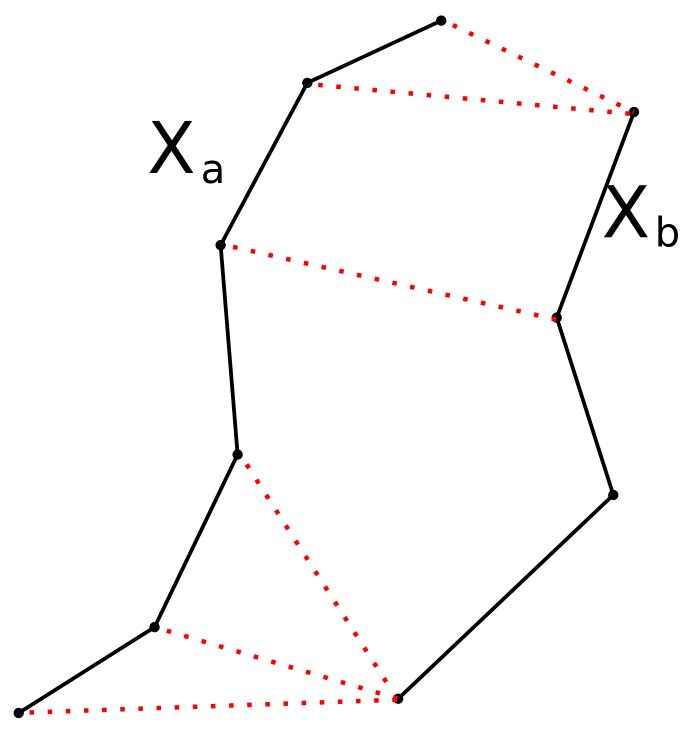
\includegraphics[width=4cm,height = 4cm]{streamline_structural_distance.pdf}
  \caption{Many distances between two streamlines, $s_A$ and $s_B$
    (solid line), that are proposed in the literature are based on the
    set of minimum distances between each point of $s_A$ to $s_B$.
    The set of minimal distances is represented here as dotted lines.}
  \label{fig:structural_distance}
\end{figure}

%\subsubsection{STAPLE sensitivity and specificity score}
%\label{subsec:experiments_quatification_staple}
%some text here

\subsubsection{Proposed method for hypotesting}
\label{subsec:experiments_quatification_proposedmethod}
From the prior knowledge of neuroscientists and doctors, there is an evidence about the reducing of the number of fibers in CST of ALS patient compared with control people. It is also the same situation with the volume of CST. Beside the number of fibers and the volume, FA and MD also play an important role for recognizing the ALS disease \cite{horsfield2002applications}. \cite{ellis1999diffusion} shows that along the corticospinal tracts, mean diffusivity was found to be significantly increased
$(p = 0.001)$ in ALS patients (limb onset: $0.771\times10^{-3} mm^2 s^{-1}$; bulbar onset: $0.778\times10^{-3} mm^2 s^{-1}$) compared with controls ($0.732\time10^{-3} mm^2 s^{-1}$). Fractional anisotropy was significantly reduced ($p = 0.007$) in bulbar onset subjects ($0.726$) compared with controls ($0.773$), but no significant difference was found between limb onset subjects ($0.761$) and controls.
Ellis et al.\cite{ellis1999diffusion} also demonstrated a positive correlation between mean diffusivity and disease duration ($r = 0.57; p = 0.009$) but no correlation with disease severity ($p > 0.29$) or upper motor neuron involvement. On the other hand, fractional anisotropy was found to correlate with measures of disease severity (assessed using the Ashworth spasticity scale and the ALS severity scale $29$).While there was no correlation between anisotropy and disease duration ($r = -0.17; p = 0.48$), significant correlations between anisotropy and the ALS severity scale ($r = -0.63; p = 0.003$) and Ashworth spasticity scale
($r = -0.56; p = 0.007$) existed.
Following are some features effectively affecting on ALS

\begin{itemize}
	\item fiber count: the number of DTI streamlines extracted for a fiber tract
	\item fiber min/max/mean length: length in $mm$ for all streamlines belonging to a fiber tract
	\item fiber volume: number of voxels occupied by all streamlines for a particular fiber tract or the geometry cylinder bounding a particular fiber tract
	\item fiber density: the ratio between fiber count and the number of voxel
	\item FA
	\item MD
	\item fragmentation: can be quantified by the ratio between the number of fibers and the volume
\end{itemize}
These features have been used as the measurement for the correctness of tractography in \cite{wang2012comprehensive}. To correct for individual differences in head size, fiber count and tract volume were normalized by intracranial volume, which was calculated from T1-weighted images using the SIENAX program in FSL \cite{smith2004techniques, smith2002accurate, smith2002automated}. 







%\input{results}

%\section{Conclusion}
\label{sec:discussion}
We implemented a software system...

%%% Local Variables: 
%%% mode: latex
%%% TeX-master: "olivetti_boi"
%%% End: 


% \input{appendix}

% conference papers do not normally have an appendix


% use section* for acknowledgement
% \section*{Acknowledgment}
% The authors would like to thank Marcel van Gerven for .


\bibliographystyle{IEEEtran}

\bibliography{ntbaovn-tract_mapping.bib}


% that's all folks
\end{document}


%%% Local Variables: 
%%% mode: latex
%%% TeX-master: "nguyen_dissimilarity"
%%% End: 







